%
% File: chap02.tex
%
\let\textcircled=\pgftextcircled
\chapter{Results}
\label{chap:result}

\initial{T}his chapter presents the results obtained during the experiment performed on September 28th, 2016. It presents the differential and integral rod worth for the transient rod, data obtained during the rod calibration. It also presents the transit time values and the maximum reactivity insertion rate of the transient rod.

\section{Rod calibration}
The fitting curve of figure~\ref{fig:int}, given by equation~\ref{eq5-int}, shows a perfect fit ($R^2 = 1$, more details on $R^2$ calculation in annexe~\ref{app:app04}) and shows an inflexion point at around 426 steps on the integral values. The fitting curve of figure~\ref{fig:diff}, on the differential points, is given by equation~\ref{eq5-diff}. It demonstrates a $R^2$ of 98\% and finds the actual inflexion point to be at around 523 steps. This goes to show that the transient rod is relatively well vertically-centered in the core, considering the uncertainties of the measurements. Indeed, the real steps in the GSTR core go from 10 to 993, hence a mid-position of 502 in the core.

\begin{figure}[t!]
	\centering
	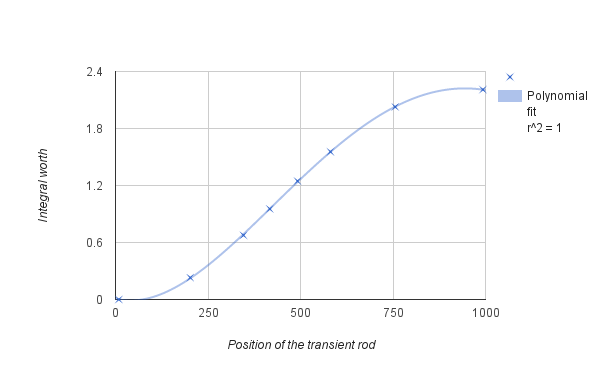
\includegraphics[height=0.4\textheight]{fig02/int.png}
	\mycaption[Integral transient rod worth]{Integral transient rod worth.}
	\label{fig:int}
\end{figure}

\begin{equation}\label{eq5-int}
y = ax^4 + bx^3 + cx^2 + dx + e
\end{equation}
Where:
\begin{conditions}
 a & $3.228 10^{-12}$ \\
 b & $- 1.242 10^{-8}$  \\
 c & $1.235 10^{-5}$ \\
 d & $- 9.536 10^{-4}$ \\
 e & $8.744 10^{-3} $
\end{conditions}

\begin{figure}[H]
	\centering
	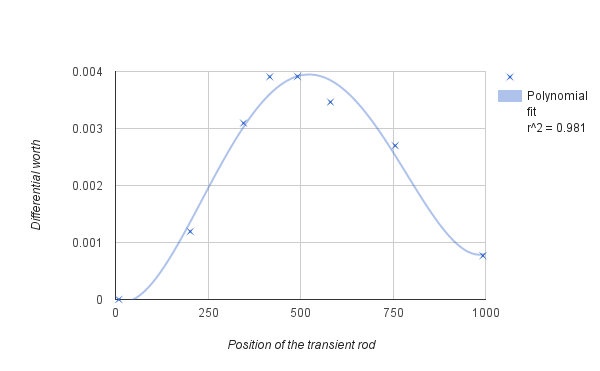
\includegraphics[height=0.4\textheight]{fig02/diff.png}
	\mycaption[Differential transient rod worth]{Differential transient rod worth.}
	\label{fig:diff}
\end{figure}

\begin{equation}\label{eq5-diff}
y = ax^4 + bx^3 + cx^2 + dx + e
\end{equation}
Where:
\begin{conditions}
 a & $6.652 10^{-14}$ \\
 b & $- 1.355 10^{-10} $ \\
 c & $7.273 10^{-8}$ \\
 d & $- 2.914 10^{-6}$ \\
 e & $-1.264 10^{-5}$ 
\end{conditions}

The transient rod can be taken from its down position to its up position in 37 seconds, meaning that in those 37 seconds, the pulse rod can introduce 2.21\$ worth of reactivity to the core. This value is below the xaximum pulse reactivity for which the reactor is licensed ($3\$$). Moreover, this means that the rod has a reactivity insertion rate of $2.21\$/37s = 0.06\$.s^{-1}$, well below the licensed limit of $0.28\$.s^{-1}$. If we consider that the rod take 1 second to fall from its top to its bottom position, this means that it introduce negative 2.21\$ worth of reactivity per second in the core.

The fact that the measured values are so far from the licensed one comes mostly from the core itself. Indeed, the fuel elements have been irradiated for a long time, and are much less energetic now that they were at the reactor's first start-up.


This experiment was performed with a "clean" core, free of Xenon poisoning. However, had it not been the case, the curves obtained would have been much different. Indeed, the Xenon would have had the effect of moving the neutron flux peak vertically in the core, moving the "center" of the core. A large Xenon poisoning, say 1.5\$, might prevent the rod calibration from being done, the differential worth being potentially negligible for some steps near the axial offset caused by the Xenon peak.




\section{Uncertainties}

Several sources of uncertainties are to be considered in this experiment. The time measurements, used to calculate the reactor period, are approximative, and probably only good within 1 second at best. The period is thus considered to be:

\begin{equation}\label{eq9}
\tau \equiv \tau \pm \frac{1}{\ln(20)} s = \tau \pm 0.33 s
\end{equation}

This translates to an approximation on the inflexion point of the integral reactivity worth of the transient rod of roughly $\pm 2$ steps. There is also an inherent uncertainty to the rod position in the core, considered equaled to one step, which means a two steps uncertainty for the differential rod worth. This translates to $\pm 1\%$ on the differential reactivity, approximately 5 steps. Thus, the updated global uncertainty on the centered position of the transient rod is $523 \pm 7$ steps, keeping in mind the fact that $R^2$ is only $98.2\%$. Moreover, the stabitlity of the nuclear power when the transient rod was pulled up was estimated using visual confirmation, introducing an uncertainty.

Other sources of uncertainties include the actual rod position measurements, the six precursor groups approximations, the $\beta_{eff}$ value, the prompt neutron lifetime, potential Xenon presence,...

All things considered, the transient rod might be very slightly off-centered, skewed toward the top of the core.
